\begin{pastexam}[label={px:nccu-113-dsa-12}]{政大資科所 113 學年度 第 12 題}
（問答）

(10\%) Consider the following binary search tree, which stores keys $a,b,c,d,e,f,g$, and $h$. Sort these
keys in non-decreasing order. For example, if you think $a\le b\le c\le d\le e\le f\le g\le h$, simply write
$a,b,c,d,e,f,g,h$.
\begin{center}
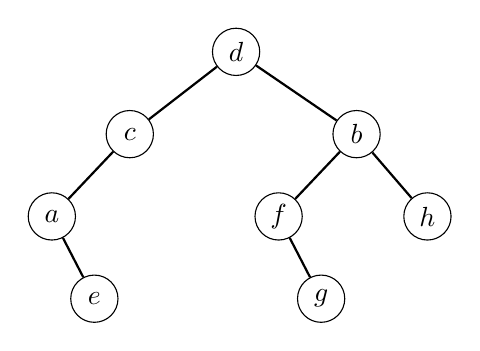
\begin{tikzpicture}[x=0.9cm,y=0.95cm,thick,tn/.style={circle,draw,thin,minimum size=6mm,inner sep=0pt}]
\node[tn] (d) at (0,0) {$d$};
\node[tn] (c) at (-1.5,-1.1) {$c$}; \node[tn] (b) at (1.7,-1.1) {$b$};
\node[tn] (a) at (-2.6,-2.2) {$a$}; \node[tn] (f) at (0.6,-2.2) {$f$}; \node[tn] (h) at (2.7,-2.2) {$h$};
\node[tn] (e) at (-2.0,-3.3) {$e$}; \node[tn] (g) at (1.2,-3.3) {$g$};
\draw (d)--(c) (d)--(b) (c)--(a) (a)--(e) (b)--(f) (b)--(h) (f)--(g);
\end{tikzpicture}
\end{center}
\end{pastexam}

\begin{pastsoln}
答案：$a, e, c, d, f, g, b, h$。

二元搜尋樹的中序走訪（左子樹、自己、右子樹）由小到大列出所有鍵（資結書定理~9.1）。 先讀出樹的結構：$d$ 是根，
左孩子 $c$、右孩子 $b$；$c$ 只有左孩子 $a$，$a$ 只有右孩子 $e$；$b$ 的左孩子 $f$、右孩子 $h$；$f$ 只有右孩子 $g$。

中序走訪：
\begin{itemize}
\item 根 $d$ 的左子樹（以 $c$ 為根）：先走 $c$ 的左子樹（以 $a$ 為根）。 $a$ 沒有左孩子，印 $a$，再走右子樹印
$e$。 回到 $c$，印 $c$；$c$ 沒有右子樹。 得 $a, e, c$。
\item 印 $d$。
\item 右子樹（以 $b$ 為根）：先走 $b$ 的左子樹（以 $f$ 為根），$f$ 沒有左孩子，印 $f$，再印右孩子 $g$。 回到 $b$
印 $b$，最後右子樹印 $h$。 得 $f, g, b, h$。
\end{itemize}
合起來是 $a \le e \le c \le d \le f \le g \le b \le h$。

檢查幾個 BST 條件：$e$ 在 $a$ 的右子樹所以 $a \le e$，又在 $c$ 的左子樹所以 $e \le c$；$g$ 在 $f$ 的右子樹、
$b$ 的左子樹，所以 $f \le g \le b$；$f, g, b, h$ 都在 $d$ 的右子樹，都 $\ge d$。 和上面的順序一致。 題目只給
樹的形狀，不同的鍵可能相等，所以寫成 $\le$；照題目要求的格式答「$a, e, c, d, f, g, b, h$」。
\end{pastsoln}
